\begin{frame}[fragile]{Potassium Channels}
\begin{tikzpicture}[scaleall=1.0]
\pcuad{\textwidth}{\textheight}
%\showcuad
\path(nw) ++(-0.5,0.25) node(corner)[graphics,anchor=north 
west]{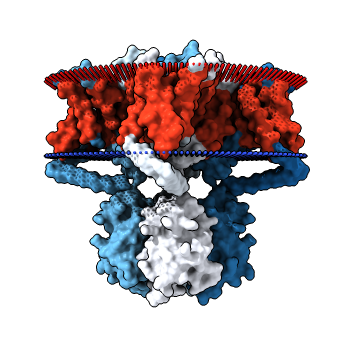
\includegraphics[width=0.33\textwidth]{2a79.png}};
\path(wp) ++(-0.0,1.0) node(corner)[graphics,anchor=north 
west]{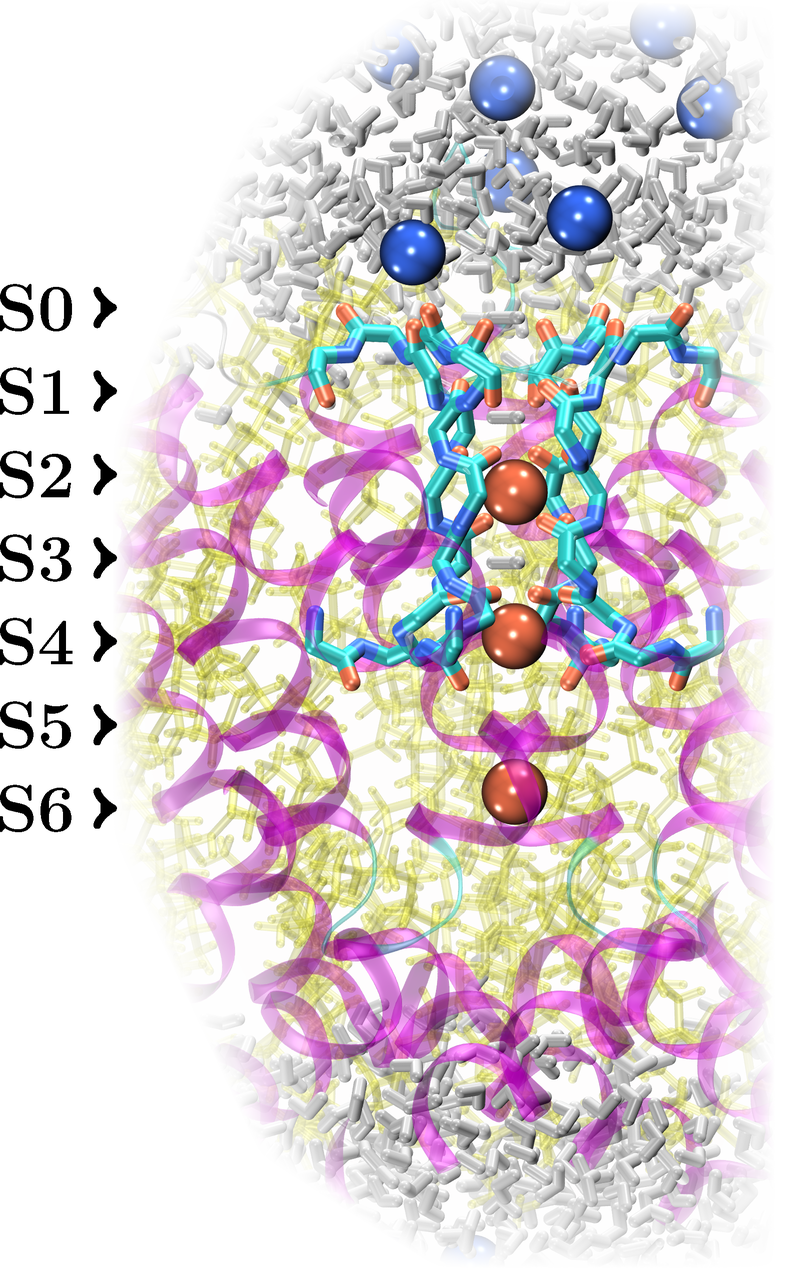
\includegraphics[width=0.25\textwidth]{Kv12_sfilter.png}};
\path(nw) ++(3,0) node(text)[anchor=north west,text width=0.75\textwidth]{
\begin{itemize}
\item Responsible for cell membrane {\em depolarization} in action-potential firing
\item Malfunctions: ``channelopathies'' like episodic ataxia, neuromyotonia, seizure, and tinnitus
\item Selectivity mechanism is not well-understood because the selectivity filter is complicated
\end{itemize}
};
\path(wp) ++(3.5,0.0) node(plot)[graphics,anchor=north west]{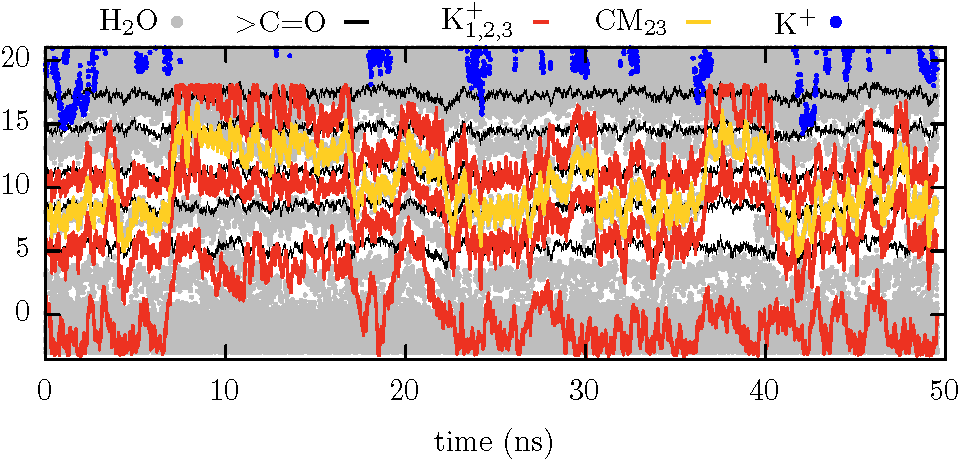
\includegraphics[width=0.65\textwidth]{fullions-crop.png}};
\end{tikzpicture}

\end{frame}

